\setlength{\columnsep}{3pt}
\begin{flushleft}

	\begin{itemize}
		\item Although there can only be \textbf{four primary partitions}, it is possible to create additional partitions.
		\item This is possible by creating an \textbf{extended partition}.
		\item An extended partition is divided up to create more partitions.
		\begin{figure}[h!]
			\centering
			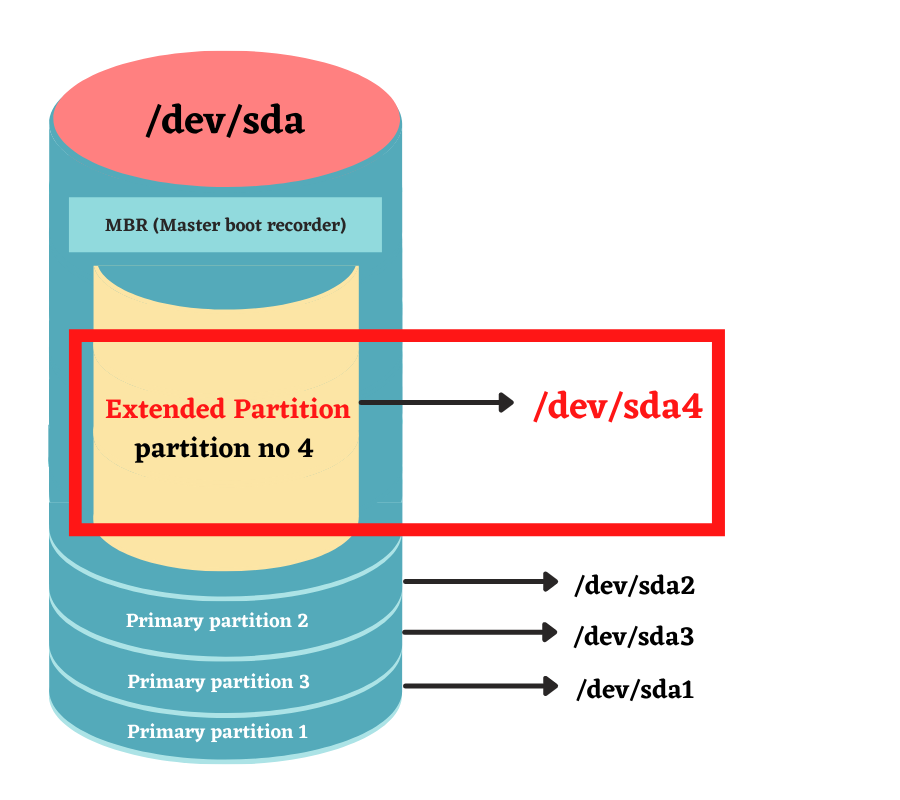
\includegraphics[scale=.6]{content/chapter8/images/ex.png}
			\caption{Extended partitions}
			\label{extended_naming}
		\end{figure}		
			\begin{tcolorbox}[breakable,notitle,boxrule=-2pt,colback=yellow,colframe=yellow]
			\color{black}
			\bigskip
			Note: Out of 4 primary partition, there can be one and only one extended partition.
			\bigskip
		\end{tcolorbox}
		
	\end{itemize}
	
\newpage

\paragraph{fdisk command option to create extended partition}

\bigskip

\begin{itemize}
	\item \textbf{e}: Create an extended partition
\end{itemize}



Eg:
\begin{figure}[h!]
	\centering
	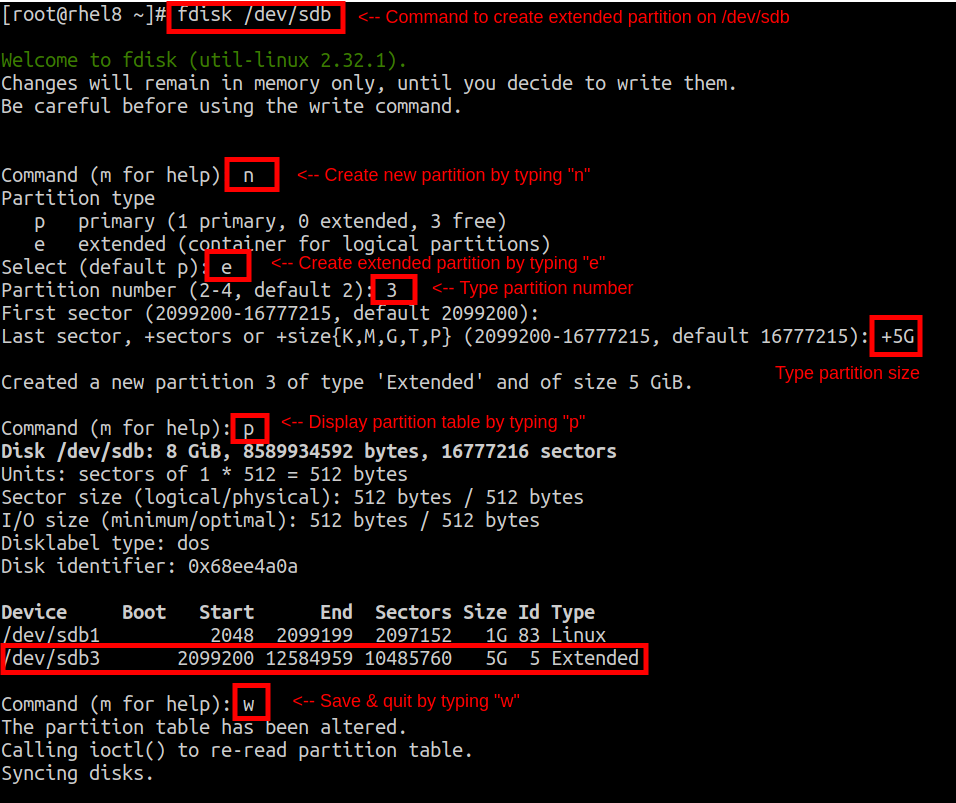
\includegraphics[scale=.4]{content/chapter8/images/extended_primary.png}
	\caption{Creating extended partitions}
	\label{primary_extended}
\end{figure}		
	
\end{flushleft}

\newpage

